
\begin{myex}

Lorsqu'un automobiliste roule à une vitesse constante, par exemple 90 km/h, la distance qu'il parcourt est proportionnelle au temps (la durée du trajet).

Les deux grandeurs proportionnelles sont \kw{le temps} en heure et \kw{la distance} parcourue e kilomètre.

\begin{multicols}{2}
	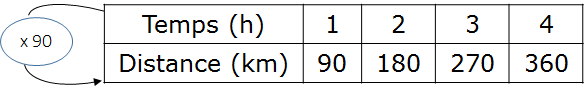
\includegraphics[scale=0.6]{img/tab1}
	
	
	{\center $\dfrac{90}{1}=\dfrac{180}{2}=\dfrac{270}{3}=\dfrac{360}{4}=90$}
\end{multicols}	
	
	On peut écrire Distance $=$ \kw{$90$}$ \: \times \:$temps, où 90 est le \kw{coefficient de proportionnalité}.
	
	\mysp
	
	\begin{center}
		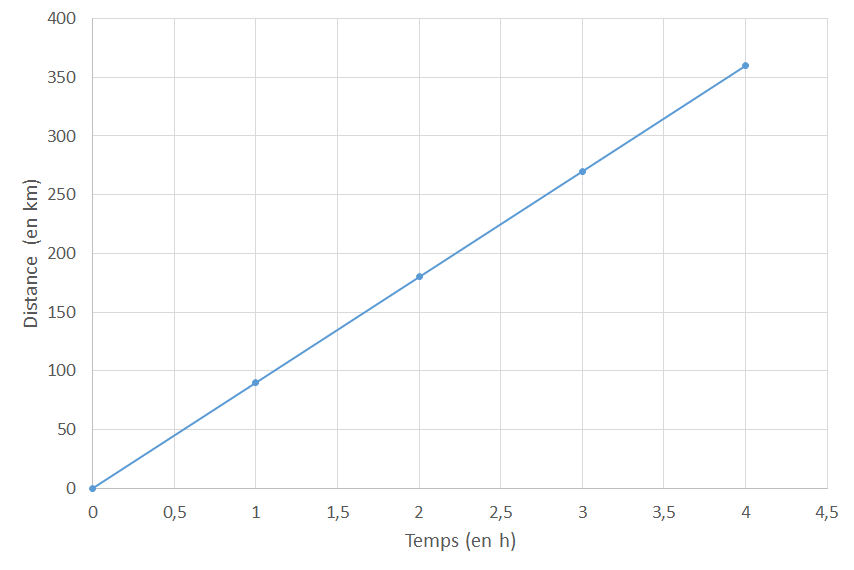
\includegraphics[scale=0.7]{img/graph1}
	\end{center}
	
	Les points de coordonnées $(temps\, ;\, distance)$ sont \kw{alignés} avec l'origine du repère.
\end{myex}